% Why far samples add bias and near samples don't --- a one-page explainer.
% Build with: tectonic -X compile locality-bias.tex --outdir build
\documentclass[11pt]{article}
\usepackage[margin=2.1cm]{geometry}
\usepackage{amsmath,amssymb}
\usepackage{tikz}
\usepackage{pgfplots}
\pgfplotsset{compat=1.18}
\usepackage{xcolor}
\usepackage{parskip}

\definecolor{accent}{HTML}{C1121F}
\definecolor{ink}{HTML}{2B2D42}
\definecolor{muted}{HTML}{6C757D}
\definecolor{good}{HTML}{2A9D8F}
\color{ink}

\newcommand{\hl}[1]{{\color{accent}\textbf{#1}}}
\newcommand{\gd}[1]{{\color{good}\textbf{#1}}}

\setlength{\parskip}{0.5em}

\begin{document}

\begin{center}
  {\LARGE\bfseries Why far samples add bias, near samples don't}\\[2pt]
  {\color{muted}\small locality and the bias of a local-average predictor (window smoother / PFN)}
\end{center}

\textbf{The setup.}
We want the true probability \emph{at the query}, $p_0(y\mid x)$.
A training point $(X_i,Y_i)$ has its label drawn from $p_0(\cdot\mid X_i)$ --- the truth \emph{at $X_i$},
which may differ from the truth at $x$. A smoother estimates $p_0(y\mid x)$ by \textbf{averaging the labels}
of the points it uses. The catch: the truth $p_0(y\mid\cdot)$ \emph{varies} across feature space (the wave below).

% ---------------------------------------------------------------- diagram ---
\begin{center}
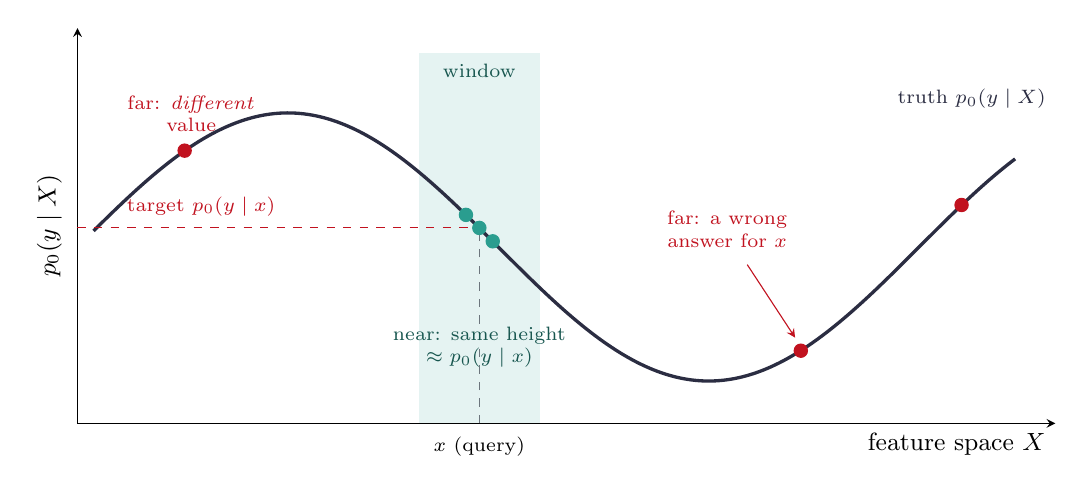
\begin{tikzpicture}
\begin{axis}[
    width=14cm, height=6.6cm,
    xlabel={feature space $X$}, ylabel={$p_0(y\mid X)$},
    xlabel style={font=\small, at={(axis description cs:1.0,0)}, anchor=north east},
    ylabel style={font=\small},
    xmin=0, xmax=7.3, ymin=0, ymax=1.12,
    axis lines=left, xtick=\empty, ytick=\empty, clip=false]

  % window around the query x = 3
  \fill[good!12] (axis cs:2.55,0) rectangle (axis cs:3.45,1.05);
  \node[good!55!black, font=\scriptsize] at (axis cs:3.0,1.0) {window};

  % the true conditional probability (a wave)
  \addplot[ink, very thick, domain=0.12:7, samples=220] {0.5+0.38*sin(deg(x))};
  \node[ink, font=\scriptsize, anchor=west] at (axis cs:6.05,0.92) {truth $p_0(y\mid X)$};

  % query x and the target value p0(y|x)
  \draw[muted, dashed] (axis cs:3,0) -- (axis cs:3,0.554);
  \node[font=\scriptsize, anchor=north] at (axis cs:3,-0.01) {$x$ (query)};
  \draw[accent, dashed] (axis cs:0,0.554) -- (axis cs:3,0.554);
  \node[accent, font=\scriptsize, anchor=south east] at (axis cs:1.55,0.56) {target $p_0(y\mid x)$};

  % NEAR samples (green) --- on the curve inside the window, same height
  \addplot[only marks, good, mark=*, mark size=2.4pt]
    coordinates {(2.9,0.591)(3.0,0.554)(3.1,0.516)};
  \node[good!55!black, font=\scriptsize, align=center, anchor=north] at (axis cs:3.0,0.30)
    {near: same height\\ $\approx p_0(y\mid x)$};

  % FAR samples (red) --- on the curve far away, very different heights
  \addplot[only marks, accent, mark=*, mark size=2.4pt]
    coordinates {(0.8,0.773)(5.4,0.206)(6.6,0.619)};
  \node[accent, font=\scriptsize, align=center, anchor=south] at (axis cs:0.85,0.80)
    {far: \emph{different}\\ value};
  \draw[accent, ->, >=stealth, shorten >=2pt] (axis cs:5.0,0.45) -- (axis cs:5.38,0.23);
  \node[accent, font=\scriptsize, align=center] at (axis cs:4.85,0.55)
    {far: a wrong\\ answer for $x$};
\end{axis}
\end{tikzpicture}
\end{center}

\textbf{Far samples $\Rightarrow$ \hl{bias}.}
A far point sits where $p_0(\cdot\mid X_{\text{far}})\neq p_0(\cdot\mid x)$ --- on a \emph{different part of the wave}.
Its label reports that different value, so averaging it in \textbf{pulls the estimate toward the wrong height}.
That is a \emph{systematic} offset --- it does not wash out no matter how much data you collect. That offset is bias.

\textbf{Near samples $\Rightarrow$ \gd{no bias}.}
If $p_0$ is smooth, a point close to $x$ has $p_0(\cdot\mid X_i)\approx p_0(\cdot\mid x)$ (same height on the wave):
its label reflects \emph{almost the same distribution we want}. Averaging near points lands on
$\approx p_0(y\mid x)$ --- no systematic offset. Shrink the window to a point and the average $\to p_0(y\mid x)$ exactly.

\textbf{The window smoother, made exact.}
For a window of radius $\theta$,
\[
  \underbrace{\mathbb E[q_\theta(y\mid x,\mathcal D_n)]-p_0(y\mid x)}_{\text{bias}}
  =\underbrace{\Pr_0\!\big(Y=y \mid \|X-x\|<\theta\big)}_{\text{average truth over the \emph{whole} window}}
  \;-\;\underbrace{p_0(y\mid x)}_{\text{truth \emph{at} }x}.
\]
A \emph{wider} window swallows more far points $\Rightarrow$ the window-average drifts further from the value at $x$
$\Rightarrow$ more bias. As $\theta\to0$, only near points survive $\Rightarrow$ bias $\to 0$.

\textbf{The trade-off (why we don't just always use near points).}
Far points are not useless: more points $=$ \emph{less variance} (noise averages out). So
\[
  \text{far points in: } \downarrow\text{variance},\ \uparrow\text{bias}
  \qquad\text{vs}\qquad
  \text{near only: } \downarrow\text{bias},\ \uparrow\text{variance}.
\]
The bandwidth is the knob. A \emph{fixed} window has constant bias; a \emph{shrinking} window ($a_n\to0$, e.g.\ $a_n=n^{-1/(4+d)}$)
drives bias $\to 0$ at the cost of fewer effective points. This is exactly why Theorem~5.4 says an \emph{unbiased}
predictor must be \hl{local} --- only near-$x$ points can be trusted.

\textbf{Everyday analogy.}
Estimate the temperature \emph{at your house} by averaging weather stations. \gd{Nearby} stations $\approx$ your
temperature (good). \hl{Distant} stations --- another city, the mountains --- have different weather, so averaging
them \emph{biases} your guess systematically.

\begin{center}
\fcolorbox{muted}{good!7}{\parbox{0.93\linewidth}{\centering
\textbf{In one line.} Far samples answer a \emph{different} question (the truth elsewhere), so averaging them
tilts your estimate away from the truth at $x$ --- that tilt is \hl{bias}. Near samples answer almost the
\emph{same} question, so they don't.}}
\end{center}

\end{document}
